%
% Copyright (c) 2011-2013, fortiss GmbH.
% Licensed under the Apache License, Version 2.0.
% 
% Use, modification and distribution are subject to the terms specified
% in the accompanying license file LICENSE.txt located at the root directory
% of this software distribution. A copy is available at
% http://chromosome.fortiss.org/.
%
% This file is part of CHROMOSOME.
%
% $Id: install_vs.tex 7852 2014-03-14 16:32:01Z geisinger $
%

\section{Installing Visual C++ 2010 Express}
\label{appx:install_vs}

Follow these steps to install Visual C++ 2010 Express:

\begin{enumerate}
	\item Point your favorite browser to
		\url{http://go.microsoft.com/?linkid=9709949}.
		This should download the web installer for Microsoft Visual C++ 2010 Express.
		If the link does not work, manually download the software:
		
		\begin{enumerate}
			\item Navigate to \url{http://www.microsoft.com/visualstudio/}
				(compare Figure~\ref{fig:setup_vs_download1}).
				Click on \emph{Download} at the top (not \emph{Download Now}!).
				In the popup menu, choose ''2012 Downloads.''

\begin{figure}[htbp]
	\centering
	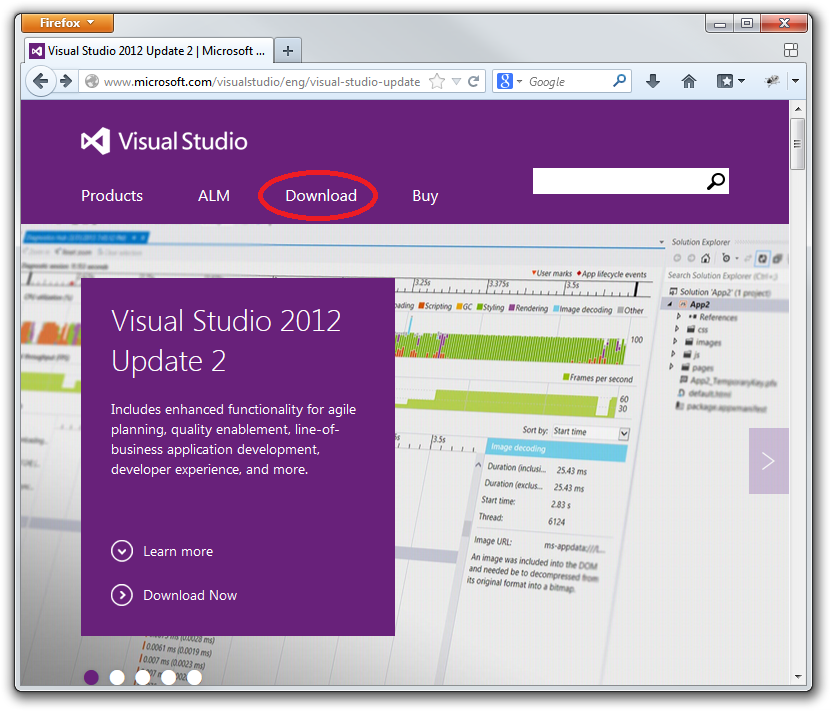
\includegraphics[scale=0.4]{figures/setup_vs_download1_edited.png}
	\caption{Manually downloading Visual C++ 2010 Express (step 1).}
	\label{fig:setup_vs_download1}
\end{figure}

			\item On the page shown in Figure~\ref{fig:setup_vs_download2},
				click on \emph{Visual Studio 2010 Express}.

\begin{figure}[htbp]
	\centering
	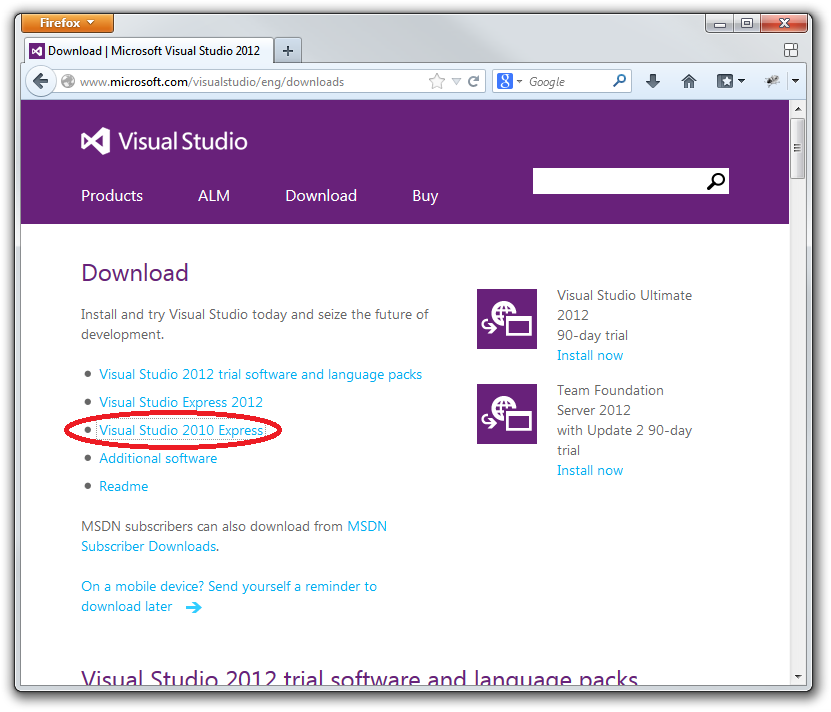
\includegraphics[scale=0.4]{figures/setup_vs_download2_edited.png}
	\caption{Manually downloading Visual C++ 2010 Express (step 2).}
	\label{fig:setup_vs_download2}
\end{figure}

			\item Open the \emph{Visual C++ 2010 Express} tab,
				choose your language and click on the arrow (compare Figure~\ref{fig:setup_vs_download3}).

\begin{figure}[htbp]
	\centering
	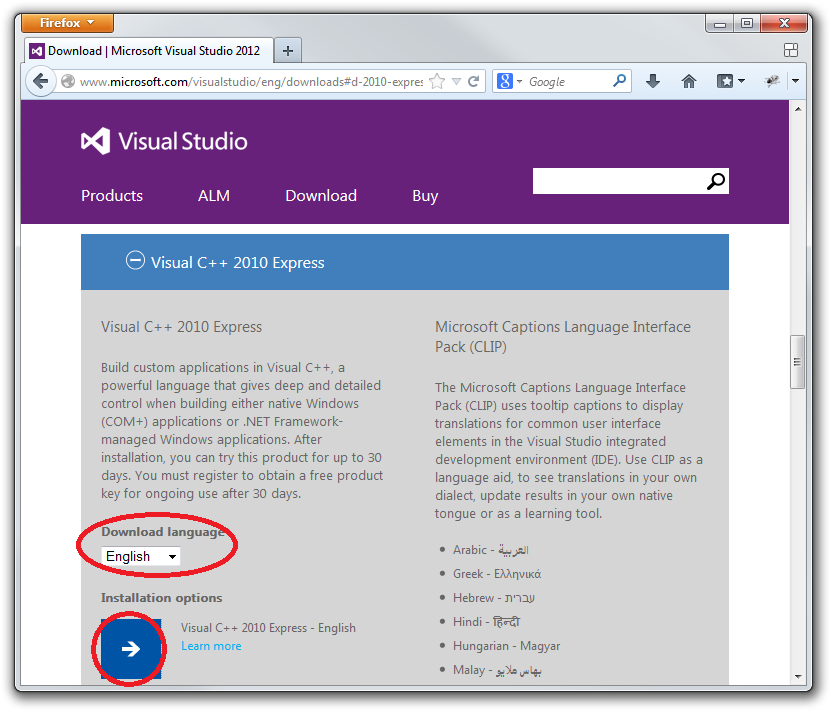
\includegraphics[scale=0.4]{figures/setup_vs_download3_edited.png}
	\caption{Manually downloading Visual C++ 2010 Express (step 3).}
	\label{fig:setup_vs_download3}
\end{figure}

			\item If you are asked whether you want to try Visual Studio Express 2012 for Windows Desktop instead,
				choose \emph{Visual C++ 2010 Express} (compare Figure~\ref{fig:setup_vs_download4}).

\begin{figure}[htbp]
	\centering
	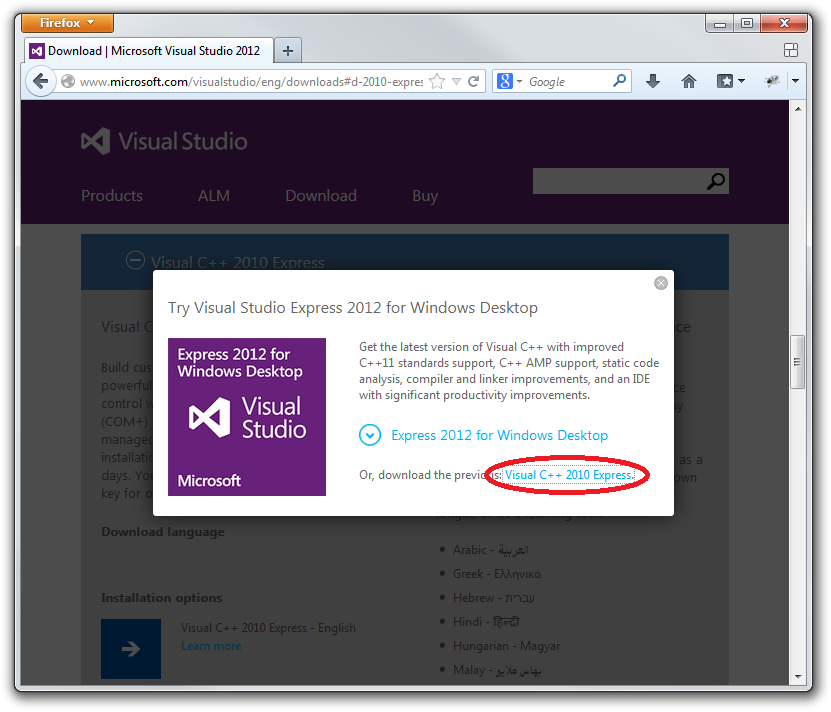
\includegraphics[scale=0.4]{figures/setup_vs_download4_edited.png}
	\caption{Manually downloading Visual C++ 2010 Express (step 4).}
	\label{fig:setup_vs_download4}
\end{figure}

		\end{enumerate}

	\item After downloading \texttt{vc\_web.exe}, launch it and follow the instructions on the screen.
		On the \emph{Installation Options} page, you may deselect \emph{Silverlight}, \emph{SQL Server 2008}
		and any related service packs; they are not needed for \xme (Figure~\ref{fig:setup_vs_optional}).

\begin{figure}[htbp]
	\centering
	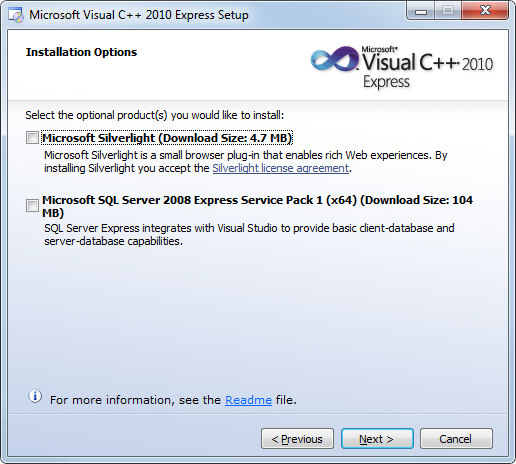
\includegraphics[scale=0.7]{figures/setup_vs_optional.png}
	\caption{Visual C++ 2010 Express installation options.}
	\label{fig:setup_vs_optional}
\end{figure}

	\item After a few minutes, \emph{Visual C++} setup will report that the installation has finished. % (Figure~\ref{fig:setup_vs_success}).
		In some cases, a reboot may be required to use \emph{Visual C++}.

\end{enumerate}
